\section{Results}
\textbf{Note}: The term indel refers to gene insertion/deletion events.
It is impossible to tell between two \ac{otu}s if a gene was deleted from one or inserted in the other, leading to an ambiguity.
Also a \ac{crsp} \ac{otu} is an \ac{otu} that I annotated as having a \ac{crsp} system as described in the methods section.
%Example Network
%Fig
\FloatBarrier
\begin{figure}[htb!]
    \makebox[\textwidth][c]{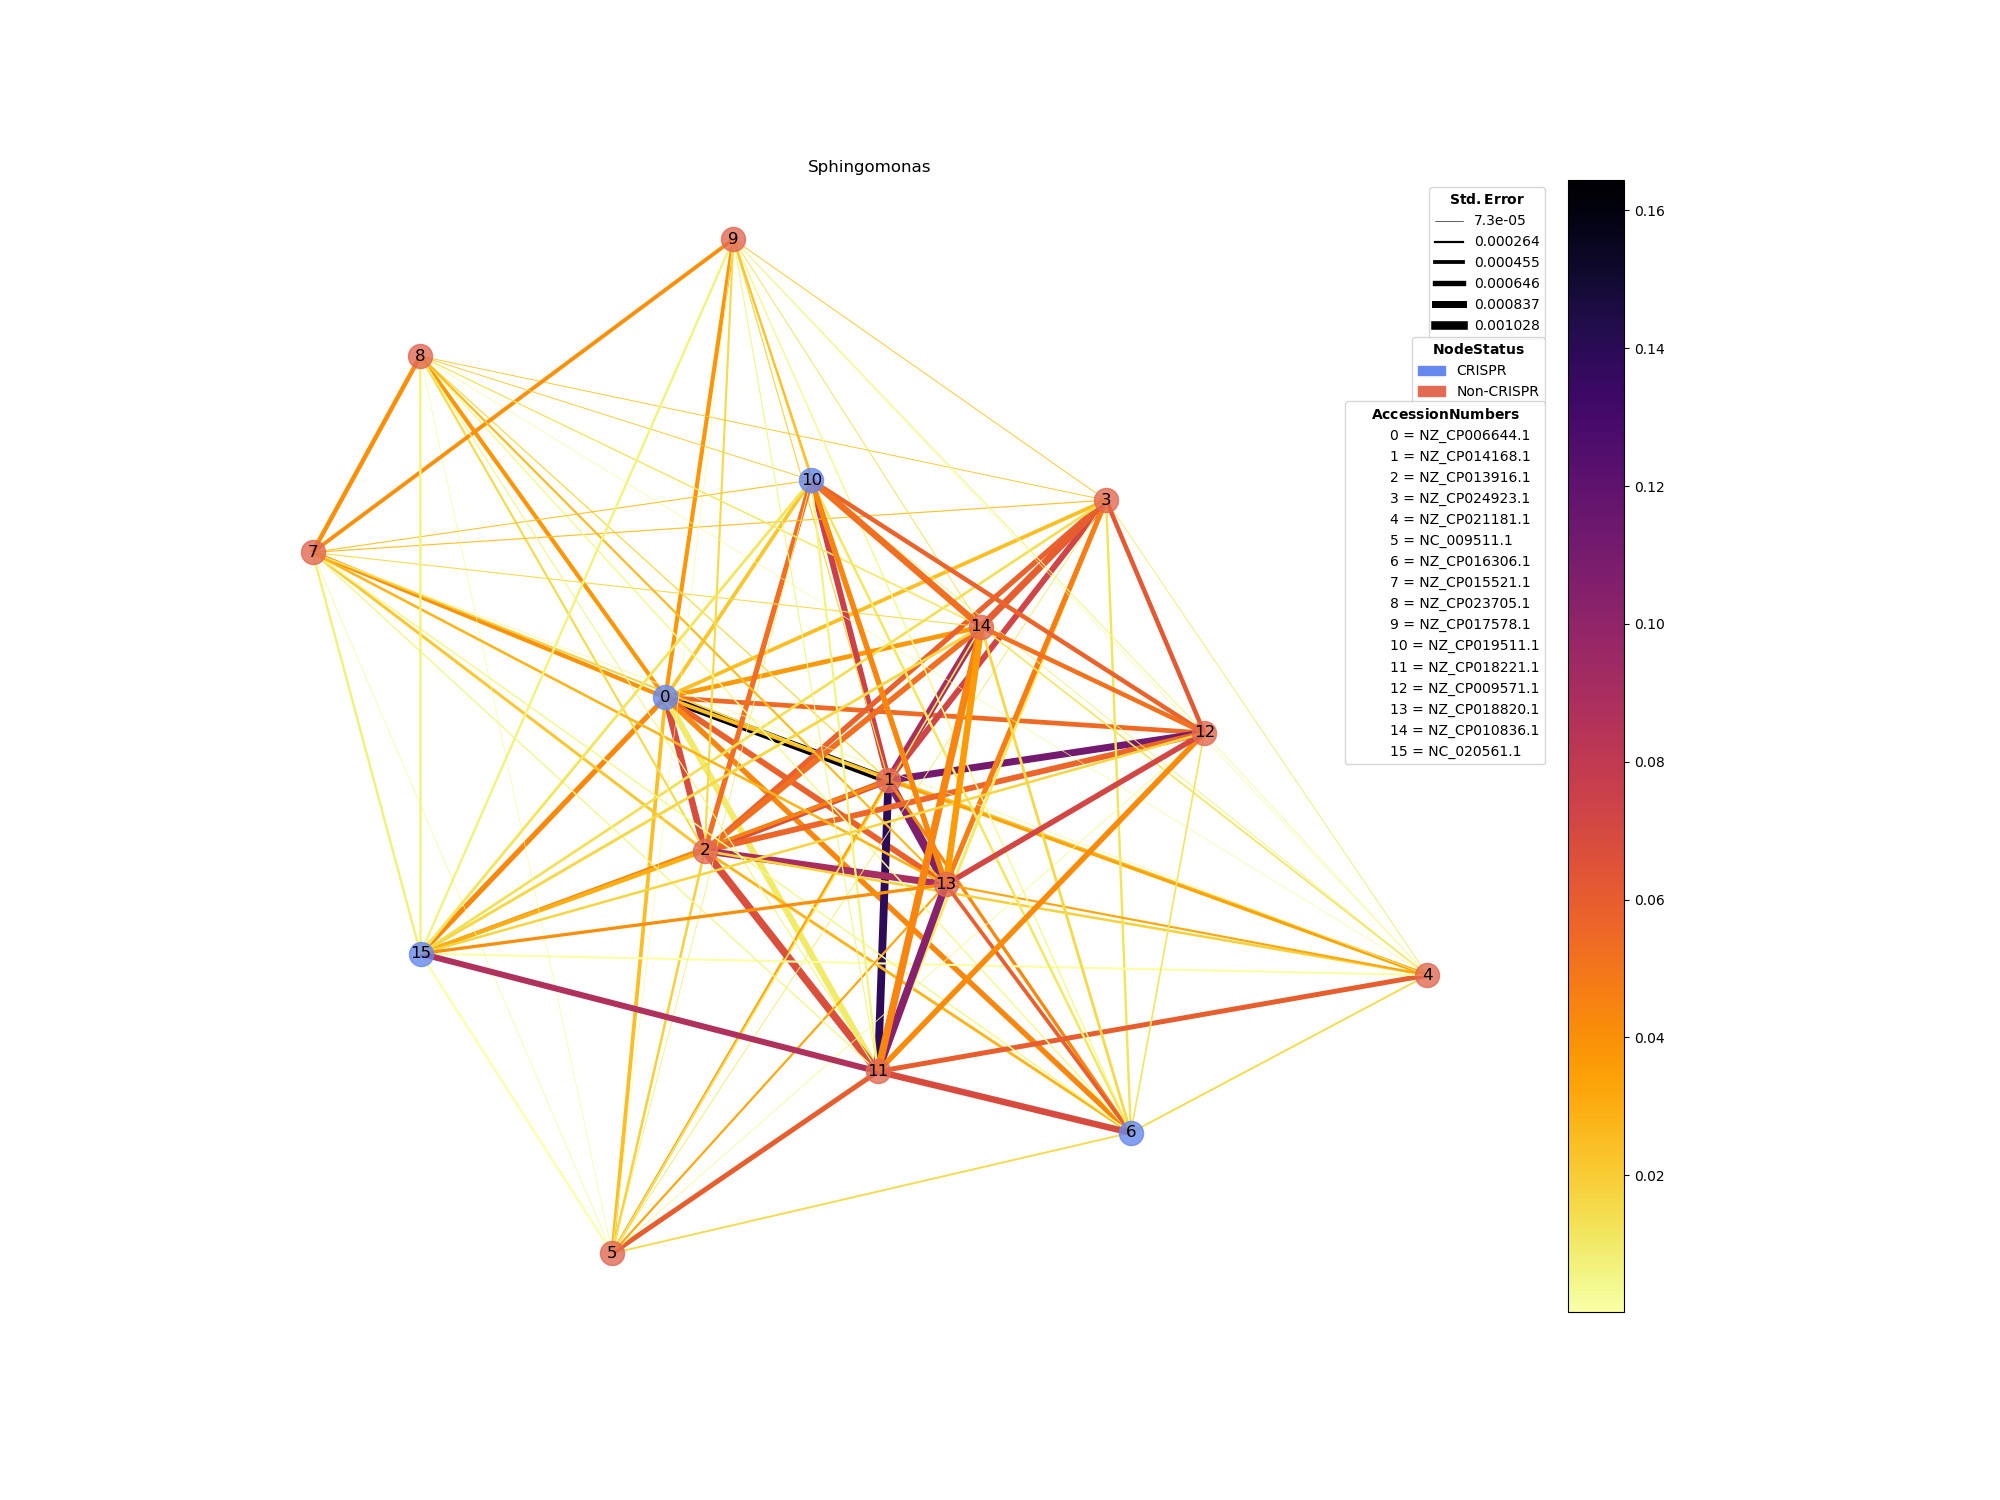
\includegraphics[width=1.3\linewidth]{network.png}}
    \caption{Example of a \ac{hgt} network produced by HiDe.
             This network is a ``consensus'' over 1000 bootstrap replicates, only including edges with a mean value $> 0$ across all bootstraps.
             Each bootstrap replicate was produced from 50 randomly sampled gene trees from a total of 376 individual gene trees.
             Blue nodes were classified as having a \ac{crsp} system, red nodes were not.
             Color represents the fraction of genes examined that were transferred along that edge.
            Width represents the standard error of the edge value over the 1000 bootstraps.
            The maximum value for an edge is 1.00, meaning all examined genes were transferred along that edge)}
    \label{net}
\end{figure}
\FloatBarrier
%Desc
In Figure \ref{net} it appears that several nodes have weak connections with most other nodes but strong connections with a few nodes.
Further both \ac{crsp} and non-\ac{crsp} nodes both show distributions of strong and weak connections with other \ac{crsp} and non-\ac{crsp} nodes both.
Also the standard error of each edge appears proportional to it's weight.
This is likely due to the sampling, as if more genes were transferred along an edge, the more likely some of those genes were left out of any individual bootstrap sample, as the size of each bootstrap sample was $\frac{50}{376}$ of the total number of gene trees.

%Genus Degree and Edge Weight Distributions
%Fig
\FloatBarrier
\begin{figure}[htb!]
    \makebox[\textwidth][c]{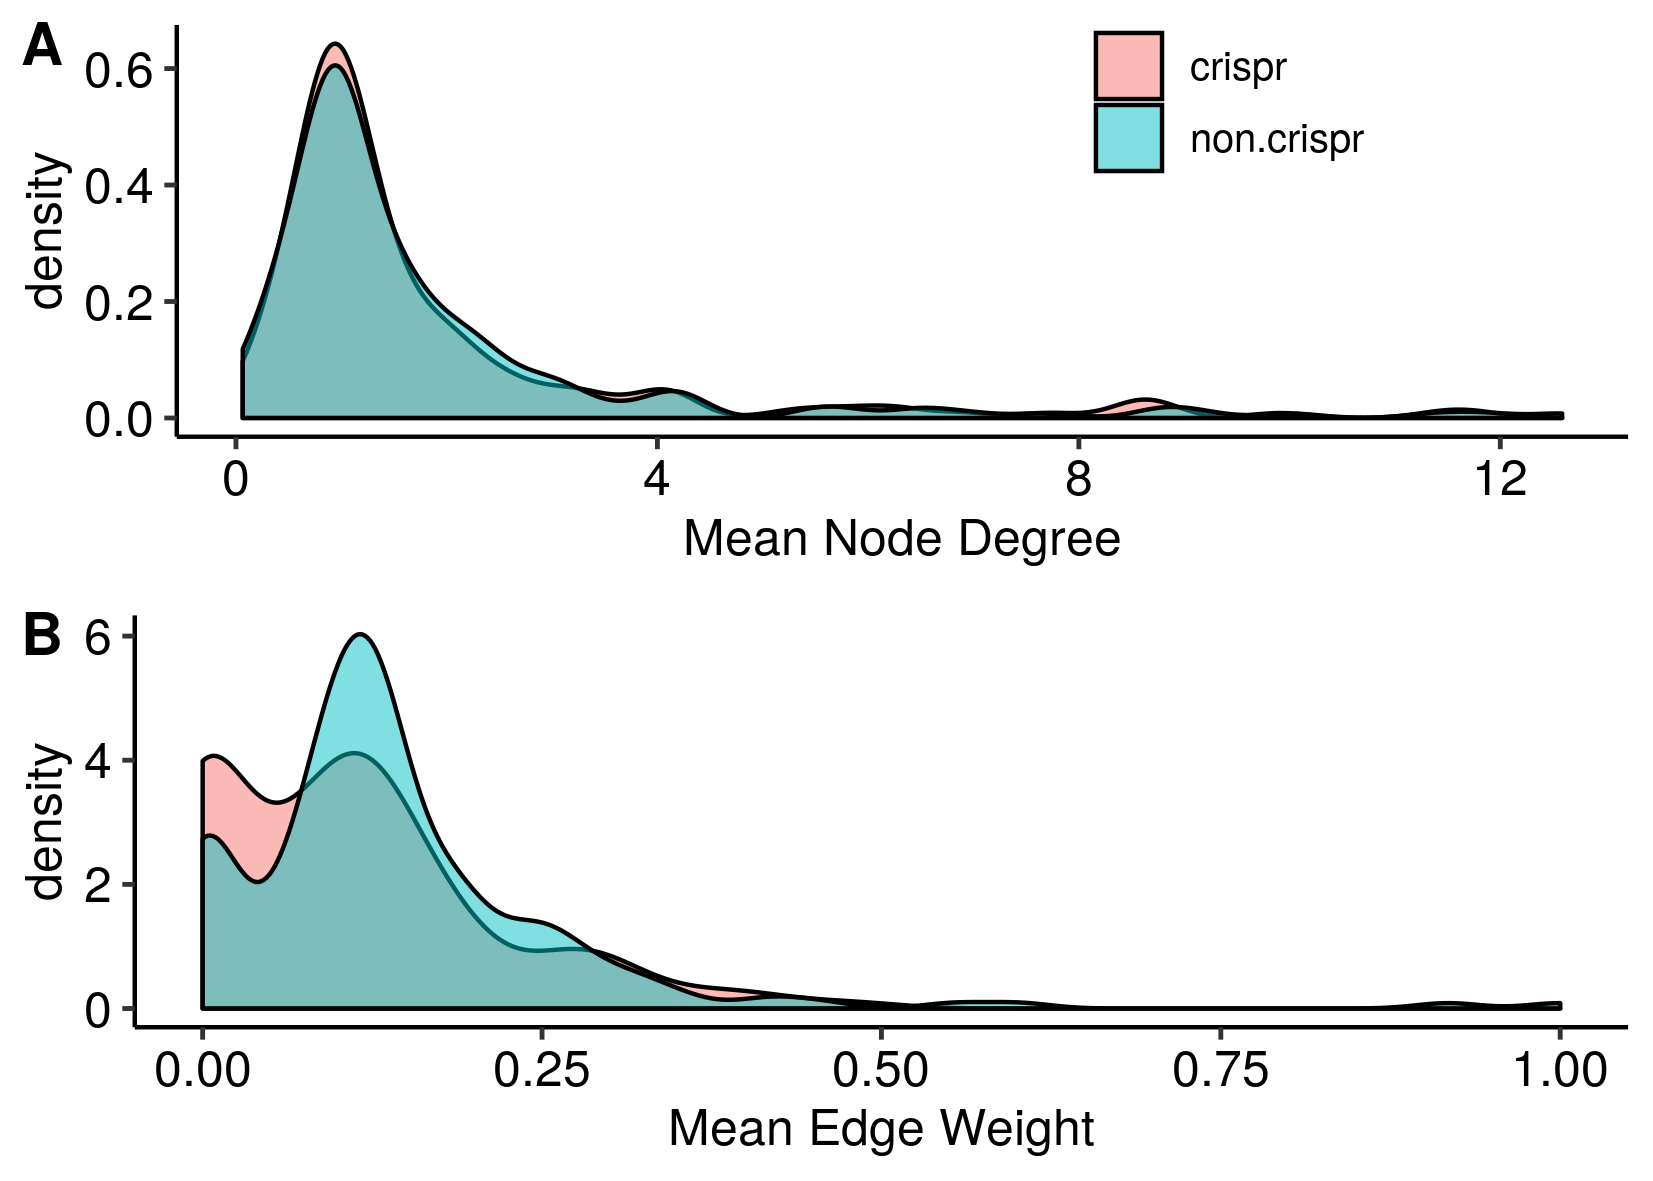
\includegraphics[width=1\linewidth]{status_vs_degree_weight.png}}
    \caption{\textbf{A)} Distribution of the degree of all nodes with/without a \ac{crsp} system. This includes the mean across all nodes in all 1000 replicates for each genus.
             \textbf{B)}  Distribution of the edge weight of all edges connected to a node with/without a \ac{crsp} system. This includes the mean across all edges in all 1000 replicates for each genus.}
    \label{degplot}
\end{figure}
\FloatBarrier
%Desc
What is immediately clear from Figure \ref{degplot} is that the node degrees are much more similar than the mean edge weights for the \ac{crsp} and non-\ac{crsp} \ac{otu}s.
This is also supported by preforming a Wilcoxon Rank Sign test comparing the \ac{crsp} and non-\ac{crsp} means.
For the mean node degree the Wilcoxon p value is 0.07412 (n=197 genera).
For the mean edge weight the Wilcoxon p value is 0.001981 (n=197 genera).
So there appears to be a significant difference between the mean edge weight for all edges but not for the degree.


%CRISPR Indel vs. Non-CRISPR Indel Scatter Plot
%Fig
\FloatBarrier
\begin{figure}[htb!]
    \makebox[\textwidth][c]{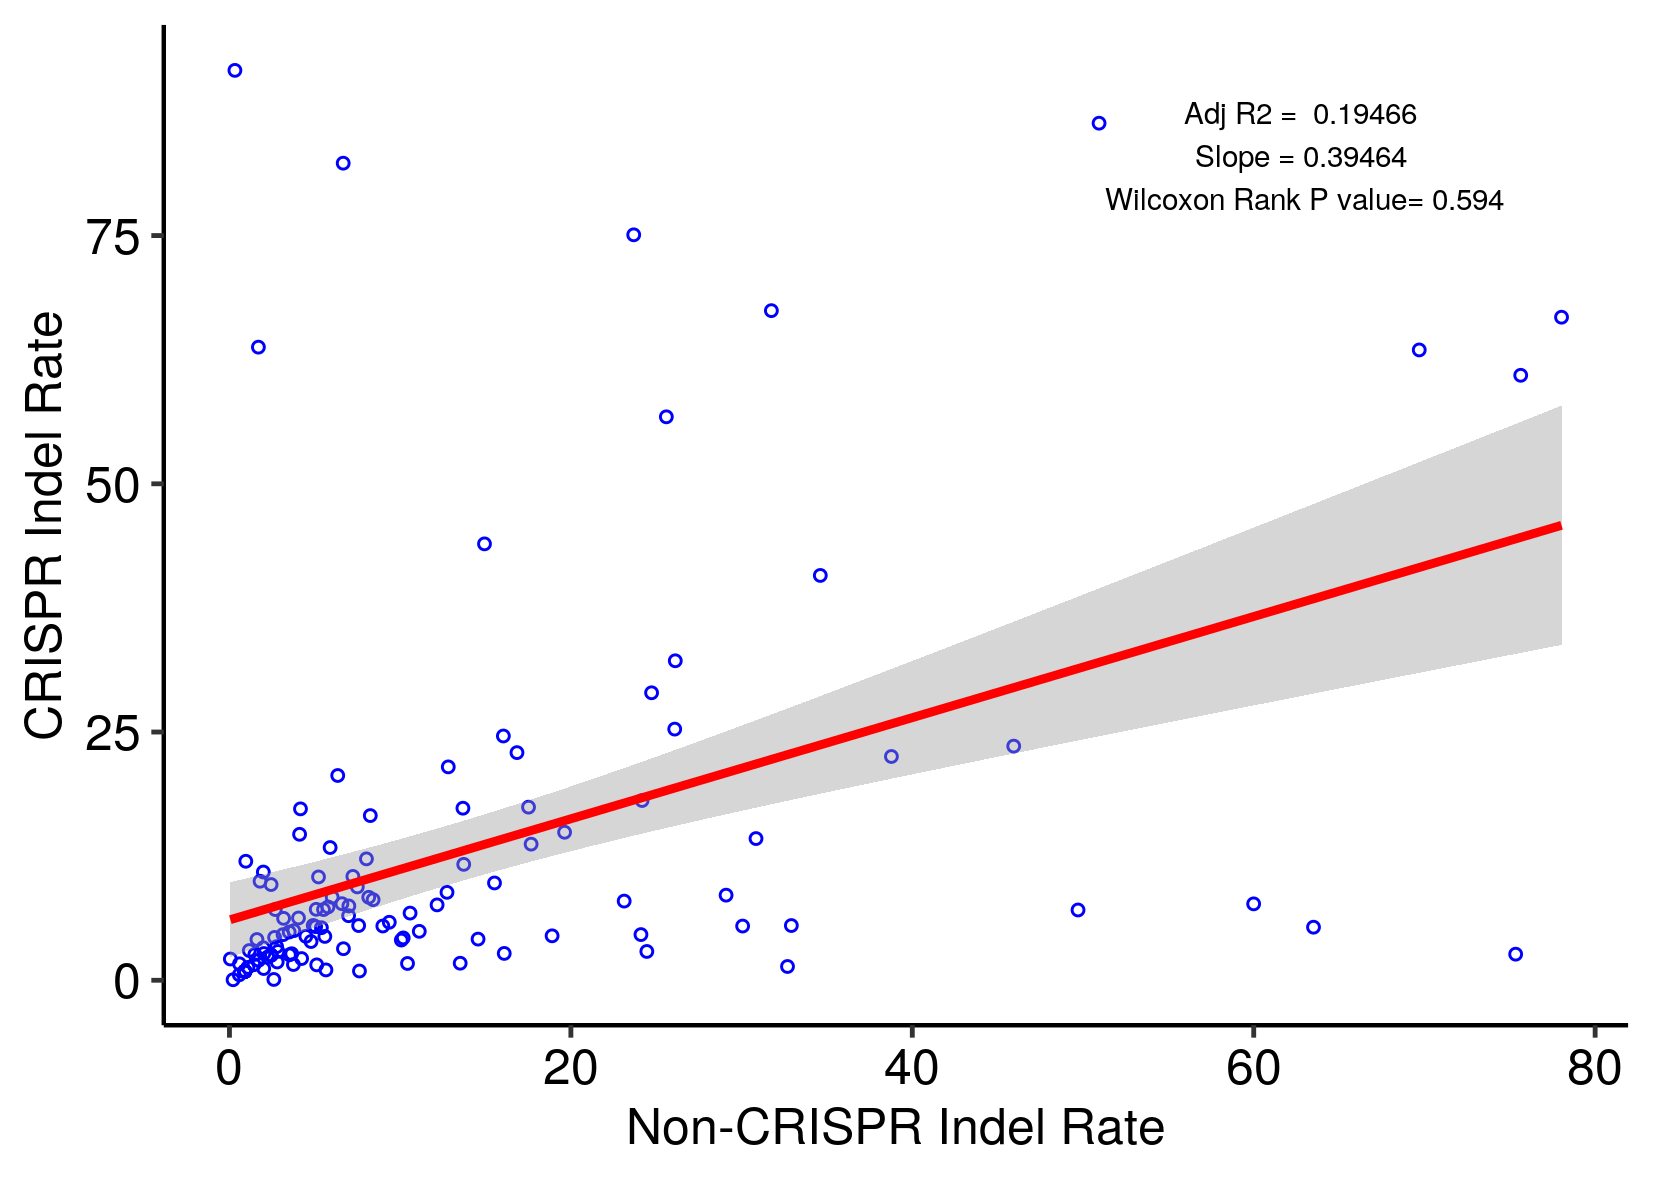
\includegraphics[width=1\linewidth]{cindel_vs_ncindel.png}}
    \caption{Markopholo estimate of gene insertion/deletion rates for the partitions of \ac{crsp} and Non-\ac{crsp} \ac{otu}s for each genus. The Rate is the number of indel events per base pair substitution. Each point represents a genus. There are 128 genera shown.}
    \label{is}
\end{figure}
\FloatBarrier
%Desc
Figure \ref{is} shows the estimated gene indel rates for the \ac{crsp} and non-\ac{crsp} branch partitions for 128 genera.
The Wilcoxon signed rank test gives a p-value of $0.594$, pointing to a lack of a significant difference in indel rates for \ac{crsp} and non-\ac{crsp} \ac{otu}s.
This is despite the fact that the slope of this fitted trend line is only 0.39464, but this may be because the trend line is influenced by specific outliers.

%CRISPR Fraction vs. Indel Rate Scatter Plot %Fig
\FloatBarrier
\begin{figure}[htb!]
    \makebox[\textwidth][c]{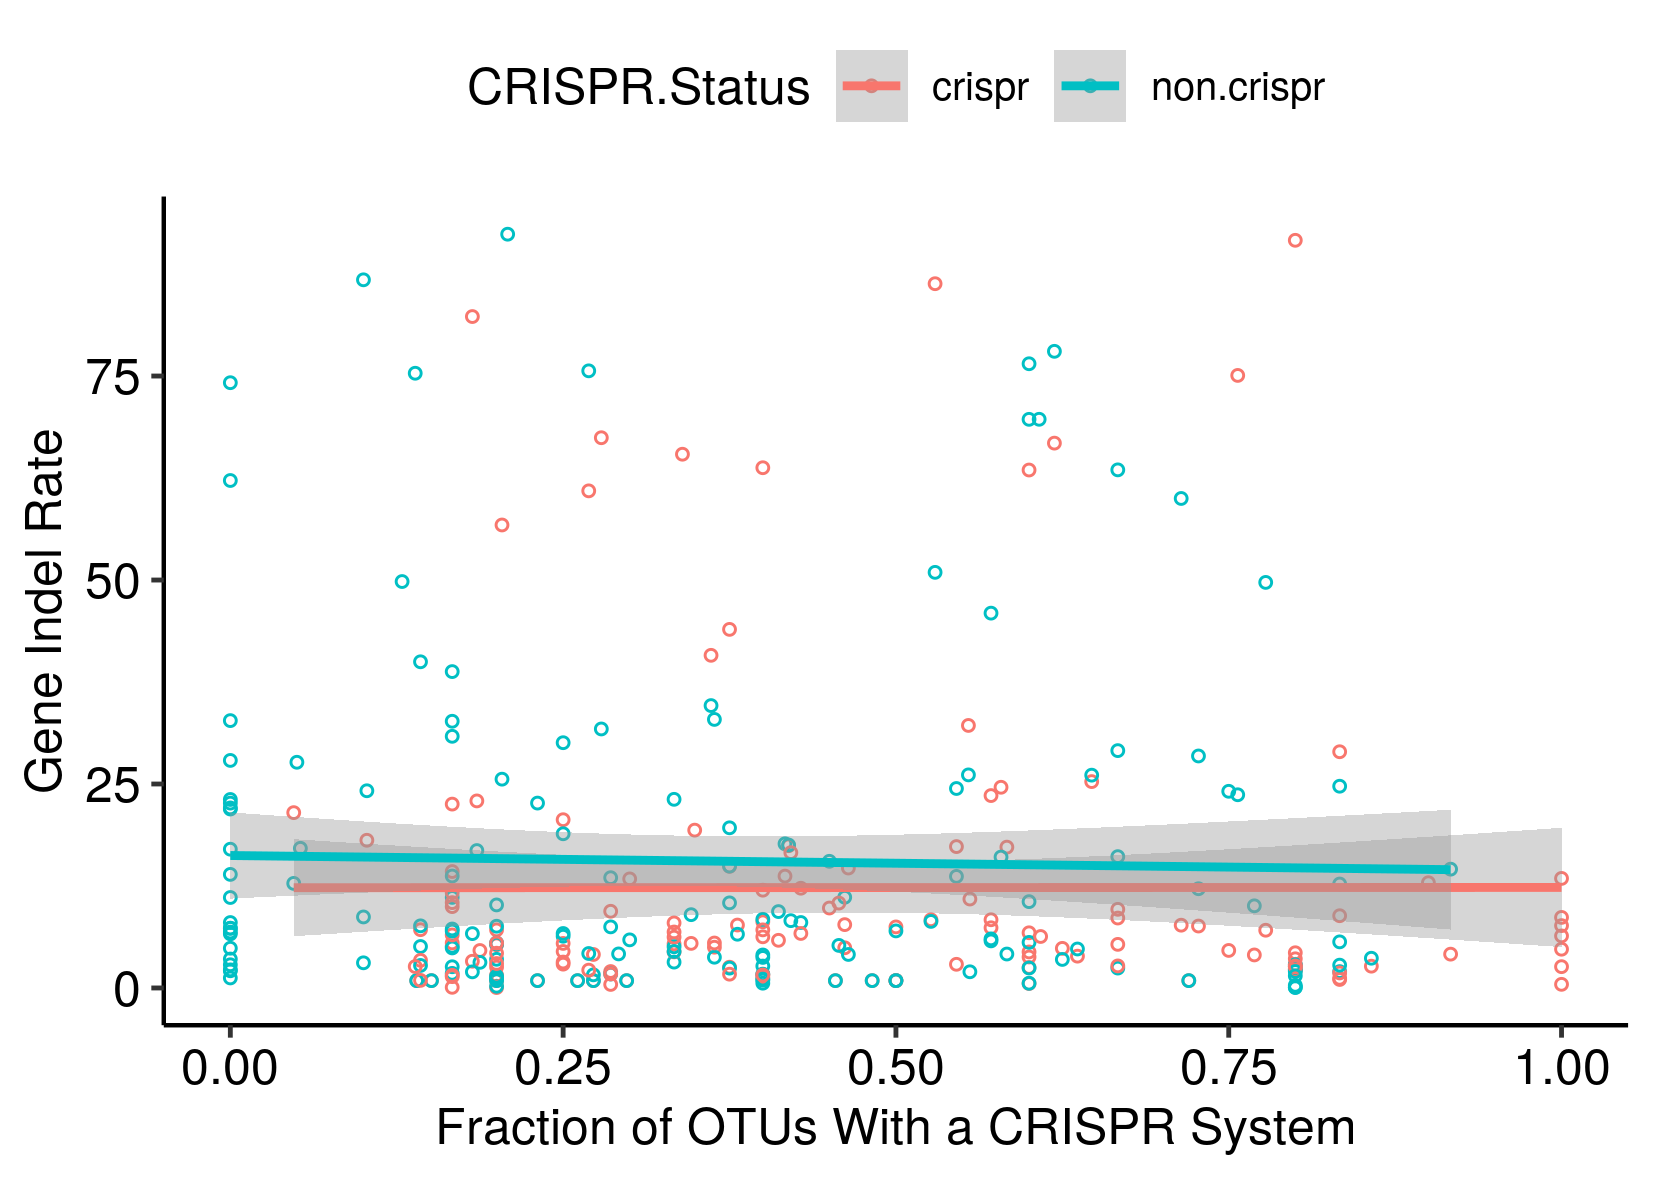
\includegraphics[width=1\linewidth]{fraction_vs_indel.png}}
    \caption{Markopholo estimate of gene indel rates for the partitions of \ac{crsp} and non-\ac{crsp} \ac{otu}s for each genus against the fraction of all \ac{otu}s in that genus that are annotated as having a \ac{crsp} system. (n=311)}
    \label{cfrd}
\end{figure}
\FloatBarrier
%Desc
Figure \ref{cfrd} show that the fraction of all \ac{otu}s in a genus with a \ac{crsp} system appears to be independent of the gene indel rate.
Neither the \ac{crsp} or non-\ac{crsp} show a relationship with \ac{crsp} fraction, having regression line slope and p values of 6.099065e-06, 0.9956342 and -0.0003156696, 0.7553688 respectively.


%Modularity and Assortativity Distributions
%Fig
\FloatBarrier
\begin{figure}[htb!]
    \makebox[\textwidth][c]{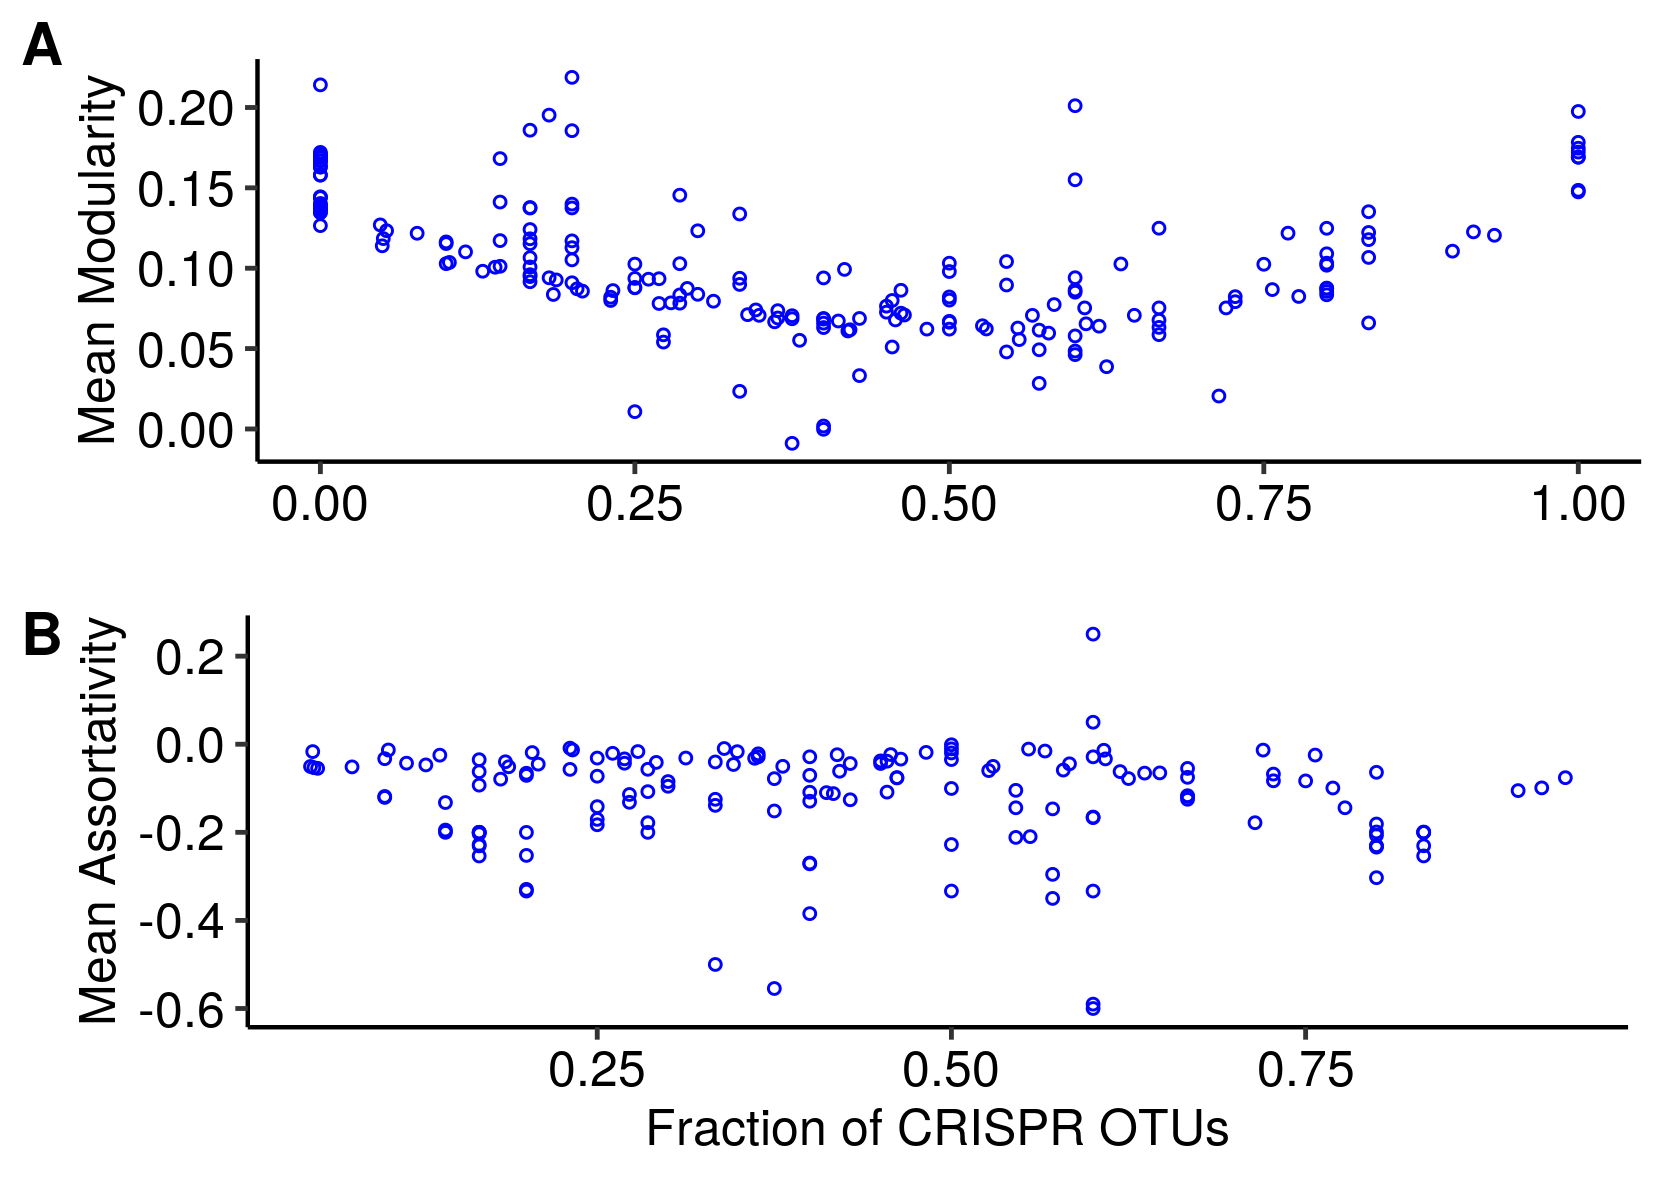
\includegraphics[width=\linewidth]{assort_and_mod.png}}
    \caption{\textbf{A)} Mean network modularity over 1000 bootstrap replicates for each genus against the fraction of all \ac{otu}s in that genera with a \ac{crsp} system  (n=197).
    \textbf{B)}  Distribution of network assortativity by \ac{crsp} status (either \ac{crsp} or non-\ac{crsp}) over 1000 bootstrap replicates for each genus against the fraction of all \ac{otu}s in that genera with a \ac{crsp} system  (n=157).}
    \label{asso_mod}
\end{figure}
\FloatBarrier
%Desc
Figure \ref{asso_mod} \textbf{A)} shows that the network modularity is centered near $0$ for most networks, implying that \ac{crsp} and non-\ac{crsp} \ac{otu}s do not form distinct communities.
There does appear to be some relationship between \ac{crsp} fraction and modularity, where the closer the \ac{crsp} fraction is to 0.5 the lower the modularity is.
This mkes intuitive sense, as if more members of the network share an attribute, the more terms are included in the sum in the definition of modularity.
Figure \ref{asso_mod} \textbf{B)} shows distribution of network assortativity is centered near $0.10$ for most networks, implying non-assortative mixing between \ac{crsp} and non-\ac{crsp} \ac{otu}s.
Assortativity is usually defined in terms of a node's degree but here node similarity is defined as whether 2 nodes are both \ac{crsp} or both non-\ac{crsp}.
This wold suggest that there is no clear separation in how \ac{crsp} and non-\ac{crsp} \ac{otu}s edges are organized in a network, with some specific exceptions.


